\documentclass[9pt,twocolumn,twoside,lineno]{pnas-new}
% Use the lineno option to display guide line numbers if required.

\templatetype{pnasresearcharticle} % Choose template 
% {pnasresearcharticle} = Template for a two-column research article
% {pnasmathematics} %= Template for a one-column mathematics article
% {pnasinvited} %= Template for a PNAS invited submission

% my stuff
\usepackage[colorinlistoftodos]{todonotes} % for comments
\usepackage{ulem}

\definecolor{red1}{RGB}{228,26,28}
\definecolor{red2}{RGB}{251,180,174}
\definecolor{blue1}{RGB}{55,126,184}
\definecolor{blue2}{RGB}{179,205,227}
\definecolor{green1}{RGB}{77,175,74}
\definecolor{green2}{RGB}{204,235,197}
% \definecolor{green3}{RGB}{166,217,106}
% \definecolor{green4}{RGB}{217,239,139}
\definecolor{purple1}{RGB}{152,78,163}
\definecolor{purple2}{RGB}{222,203,228}
\definecolor{orange1}{RGB}{255,127,0}
\definecolor{orange2}{RGB}{254,217,166}
\definecolor{mustard1}{RGB}{191,129,45}
\definecolor{mustard2}{RGB}{254,217,118}
% \definecolor{brown1}{RGB}{166,86,40}
% \definecolor{brown2}{RGB}{229,216,189}
% \definecolor{pink1}{RGB}{247,129,191}
% \definecolor{pink2}{RGB}{253,218,236}
% \definecolor{gray1}{RGB}{115,115,115}
% \definecolor{gray2}{RGB}{153,153,153}
\definecolor{blueish}{RGB}{103,169,207}
\definecolor{greenish}{RGB}{161,217,155}

\newcommand{\SCP}[2]{\textcolor{red2}{\sout{#1}}\textcolor{red1}{#2}} % Sam
\newcommand{\TC}[2]{\textcolor{blue2}{\sout{#1}}\textcolor{blue1}{#2}} % Tommy
\newcommand{\SP}[2]{\textcolor{green2}{\sout{#1}}\textcolor{green1}{#2}} % Simona
\newcommand{\RJ}[2]{\textcolor{purple2}{\sout{#1}}\textcolor{purple1}{#2}} % Rocío
\newcommand{\MRB}[2]{\textcolor{orange2}{\sout{#1}}\textcolor{orange1}{#2}} % Mathieu
\newcommand{\MEB}[2]{\textcolor{mustard2}{\sout{#1}}\textcolor{mustard1}{#2}} % Matt
% \newcommand{\JA}[2]{\textcolor{brown2}{\sout{#1}}\textcolor{brown1}{#2}} % Jelle
% \newcommand{\SCT}[2]{\textcolor{pink2}{\sout{#1}}\textcolor{pink1}{#2}} % Susana
% \newcommand{\ODO}[2]{\textcolor{gray2}{\sout{#1}}\textcolor{gray1}{#2}} % Ollie
% \newcommand{\JZ}[2]{\textcolor{green4}{\sout{#1}}\textcolor{green3}{#2}} % Jeff



\title{Trends and gaps in a decade of movement ecology}

% Use letters for affiliations, numbers to show equal authorship (if applicable) and to indicate the corresponding author
\author[a,2]{Rocío Joo}
\author[a]{Simona Picardi} 
\author[b,1]{Thomas A. Clay}
\author[a,1]{Matthew E. Boone} 
\author[b]{Samantha C. Patrick} 
\author[a]{Mathieu Basille} 

\affil[a]{Department of Wildlife Ecology and Conservation, Fort Lauderdale Research and Education Center, University of Florida, Fort Lauderdale, FL, USA}
\affil[b]{School of Environmental Sciences, University of Liverpool, Liverpool, UK}

% Please give the surname of the lead author for the running footer
\leadauthor{Joo} 

% Please add here a significance statement to explain the relevance of your work
\significancestatement{Authors must submit a 120-word maximum statement about the significance of their research paper written at a level understandable to an undergraduate educated scientist outside their field of speciality. The primary goal of the Significance Statement is to explain the relevance of the work in broad context to a broad readership. The Significance Statement appears in the paper itself and is required for all research papers.}

% Please include corresponding author, author contribution and author declaration information
\authorcontributions{Please provide details of author contributions here.}
\authordeclaration{Please declare any conflict of interest here.}
\equalauthors{\textsuperscript{1}A.O.(Author One) and A.T. (Author Two) contributed equally to this work (remove if not applicable).}
\correspondingauthor{\textsuperscript{2}To whom correspondence should be addressed. E-mail: author.two\@email.com}

% Keywords are not mandatory, but authors are strongly encouraged to provide them. If provided, please include two to five keywords, separated by the pipe symbol, e.g:
\keywords{Keyword 1 $|$ Keyword 2 $|$ Keyword 3 $|$ ...} 

\begin{abstract}
<250 words for abstract. I had an idea for the abstract but I forgot my little notebook where I wrote it...
\end{abstract}

\dates{This manuscript was compiled on \today}
\doi{\url{www.pnas.org/cgi/doi/10.1073/pnas.XXXXXXXXXX}}

\begin{document}

\maketitle
\thispagestyle{firststyle}
\ifthenelse{\boolean{shortarticle}}{\ifthenelse{\boolean{singlecolumn}}{\abscontentformatted}{\abscontent}}{}

% If your first paragraph (i.e. with the \dropcap) contains a list environment (quote, quotation, theorem, definition, enumerate, itemize...), the line after the list may have some extra indentation. If this is the case, add \parshape=0 to the end of the list environment.
\dropcap{T}his section would be an introduction to movement ecology and the advances in the last 10 years. \todo[color=blueish!20]{RJ: Reminding that it's about movement of whole organisms.} We'd mention the movement ecology special issue in PNAS, and particularly Nathan's paper in 2008 with the framework (or paradigm; we'll call it MEP as in other publications). Shortly describe Holyoak's paper in 2008 quantifying studies of movement and MEP by taxon. Some important things the paper says: There was a lack of studies of the different components of the MEP  (most studies were describing movement and how it's influenced by the environment, conspecifics or others, but "we rarely know why spaces follow particular movement paths and how their mode of movement relates to short-term and long-term costs and benefits"), and called for more integrative (interdisciplinary) studies. They also mentioned some differences in taxa (studying movement), though they measure something different than us. 

The idea of the paper is to assess the state of the field of movement ecology after Nathan's seminal paper and the special issue, by analyzing the text of all peer-reviewed scientific articles published between 2009 and 2018. We focus on several key aspects: the questions (express through the MEP), the species studied, the data collection, the software and the methods for analysis. Fig.1 represents the implicit dependencies between aspects (e.g. the choice of methods depend on the type of data to analyze). Generally speaking, movement ecology studies could be classified as organism-centered (i.e. the main goal is the gain of knowledge about a species) or process-centered (i.e. the main goal is to understand the processes behind movement in general: why, how, when and where movement is produced, and the organisms studied is a tool to get to that knowledge). We examine these two aspects (questions and species) first, as they are the main focus of movement ecology. \todo[color=blueish!20]{RJ: This is just my personal view. Also, I don't use this much in the paper so we could delete it.} Then, we assess the other three aspects and their connections with the questions and species. We also review and discuss how interdisciplinary is the field now and the challenges that we face now as a research community.

The statistics shown in this work were a result of the text analysis of 4417 movement ecology papers published between 2009 and 2018. The methods for selecting the papers and extracting the information are described in Supp. Mat. 1. We also conducted an online survey on movement ecologists asking about their perception of the field (Supp. Mat. 2). These perceptions are discussed in the following sections. 

\begin{figure}%[tbhp]
\centering
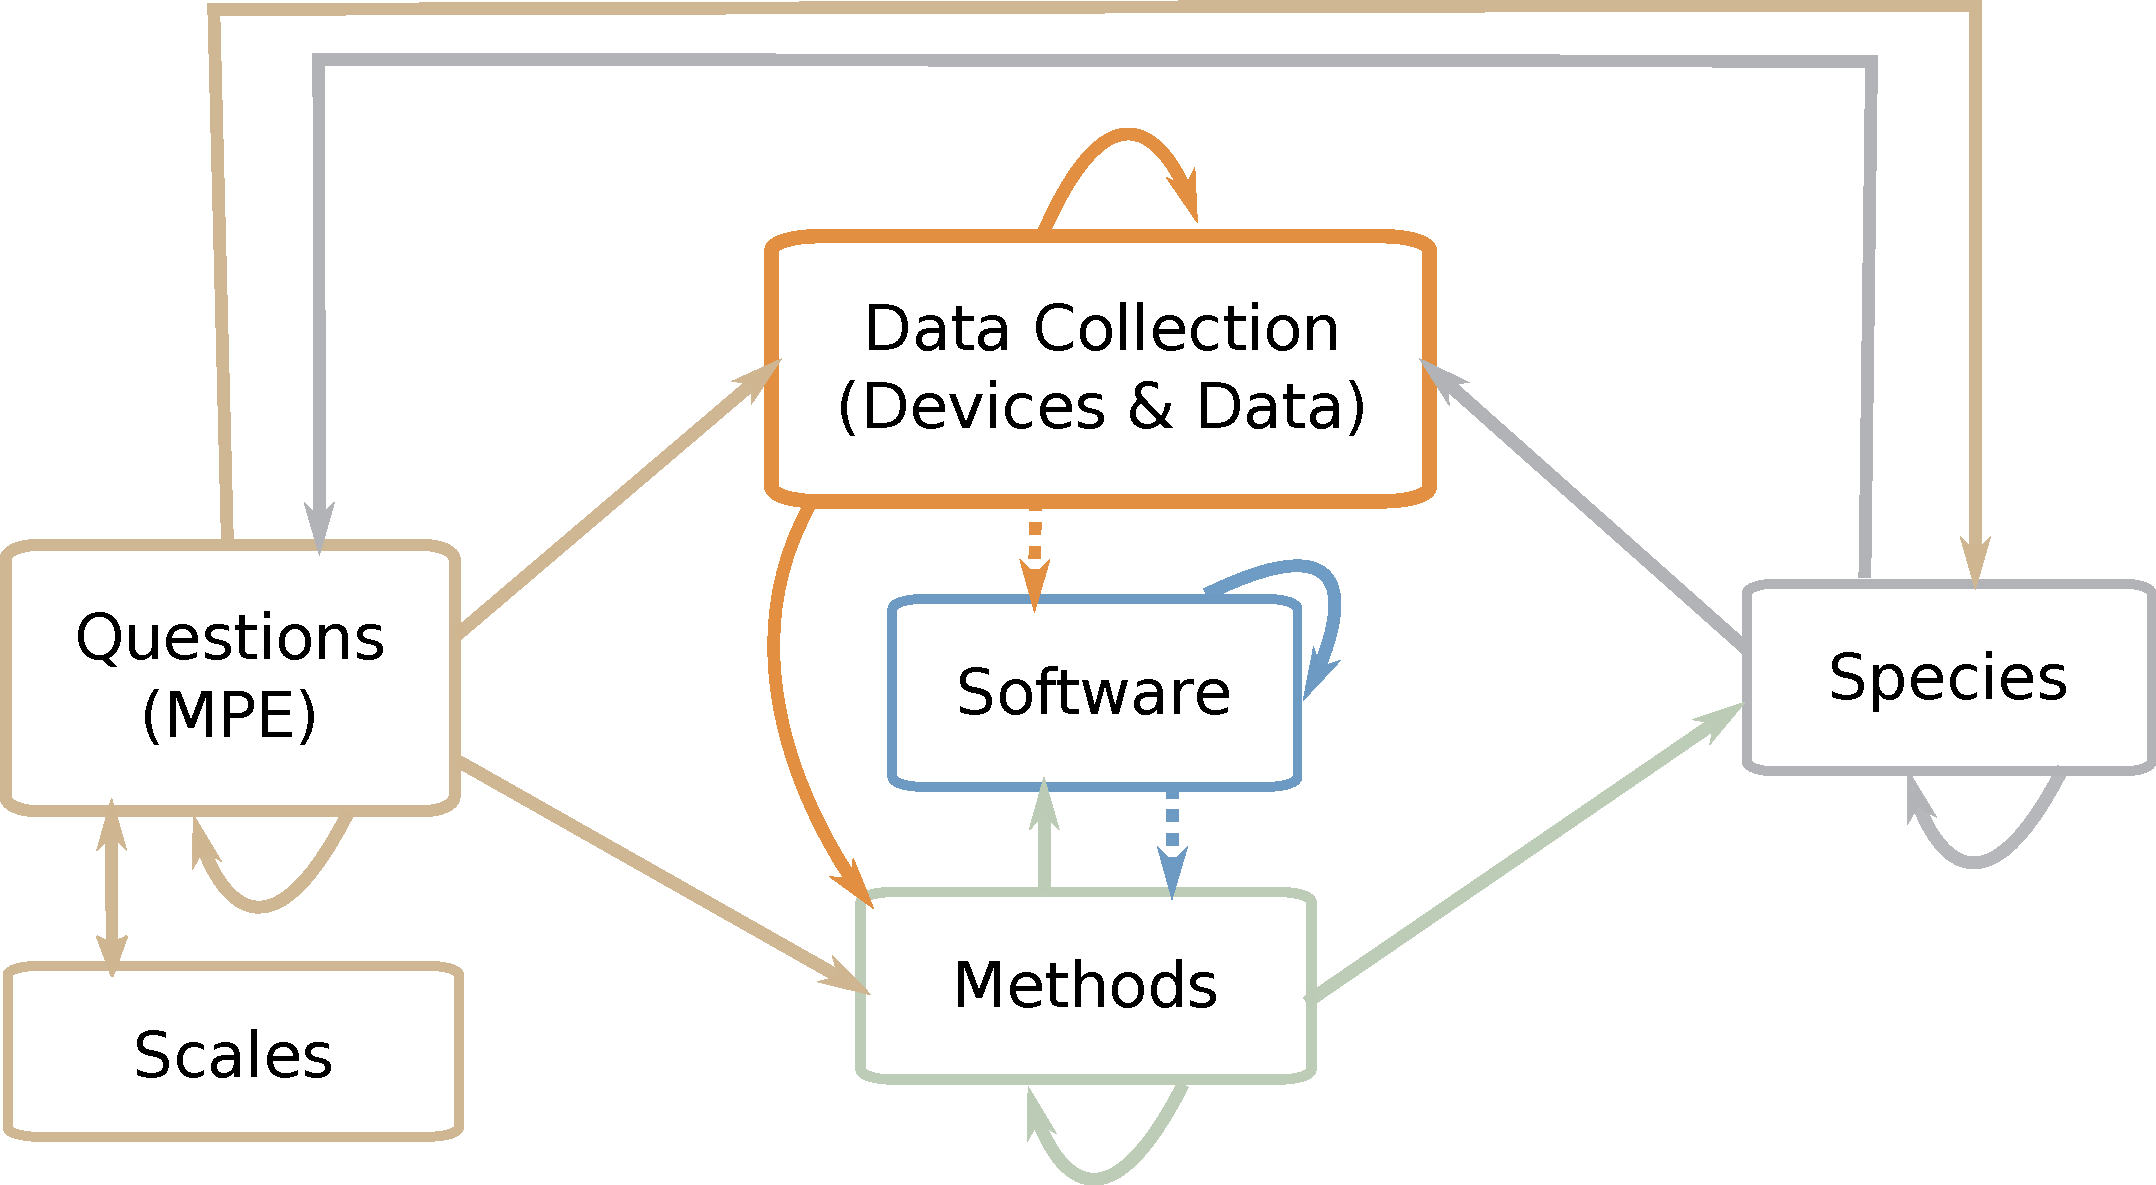
\includegraphics[width=.8\linewidth]{./img/DimensionsFrame.pdf}
\caption{Key aspects for movement ecology: questions (represented by the movement ecology paradigm), species, data collection, software and methods for analysis. The questions have to take into account scales of movement. The arrows depart from the aspect that is needed to make a decision on the aspect at the other end of the arrow. Circular arrows indicate that this aspect can also be chosen by itself (e.g. the researcher's preference). Dotted arrows indicate some links that often happen but should not: the software is chosen because it is `good' for some kind of data, or the methods are chosen because they are available in a software.}
\label{fig:aspects}
\end{figure}

\section*{The movement ecology paradigm: are we forgetting about the processes?}

- Introduction to the MEP and the questions behind it (I think "why" is not only related to internal but also external factor. And so is when)\todo[color=blueish!20]{RJ: Does everyone agree on that?}. And scales. 
- Mention the number of papers that refer to the movement ecology paradigm (or framework). Number of papers with scales in KAT (keywords, abstract, title) \todo[color=blueish!20]{RJ: I still need to do that.} 
- Fig. 2: MEP and quantification of the links between components. This is tricky because the dictionaries were created for motion and navigation processes and not capacities. 
- Table 1: main "keywords" or categories for each component. 
- Discuss those results. We are still like in Holoyak's paper: mostly caring about external factor's role in movement. Why? Is everything else so difficult to quantify? Is it difficult to get data on motion or navigation? Are the methods not good for that? Are we not working with physiologists or physicists enough? (Invite to check next sections). Discuss "scale results".
- Add stuff from the survey.

\begin{figure}%[tbhp]
\centering
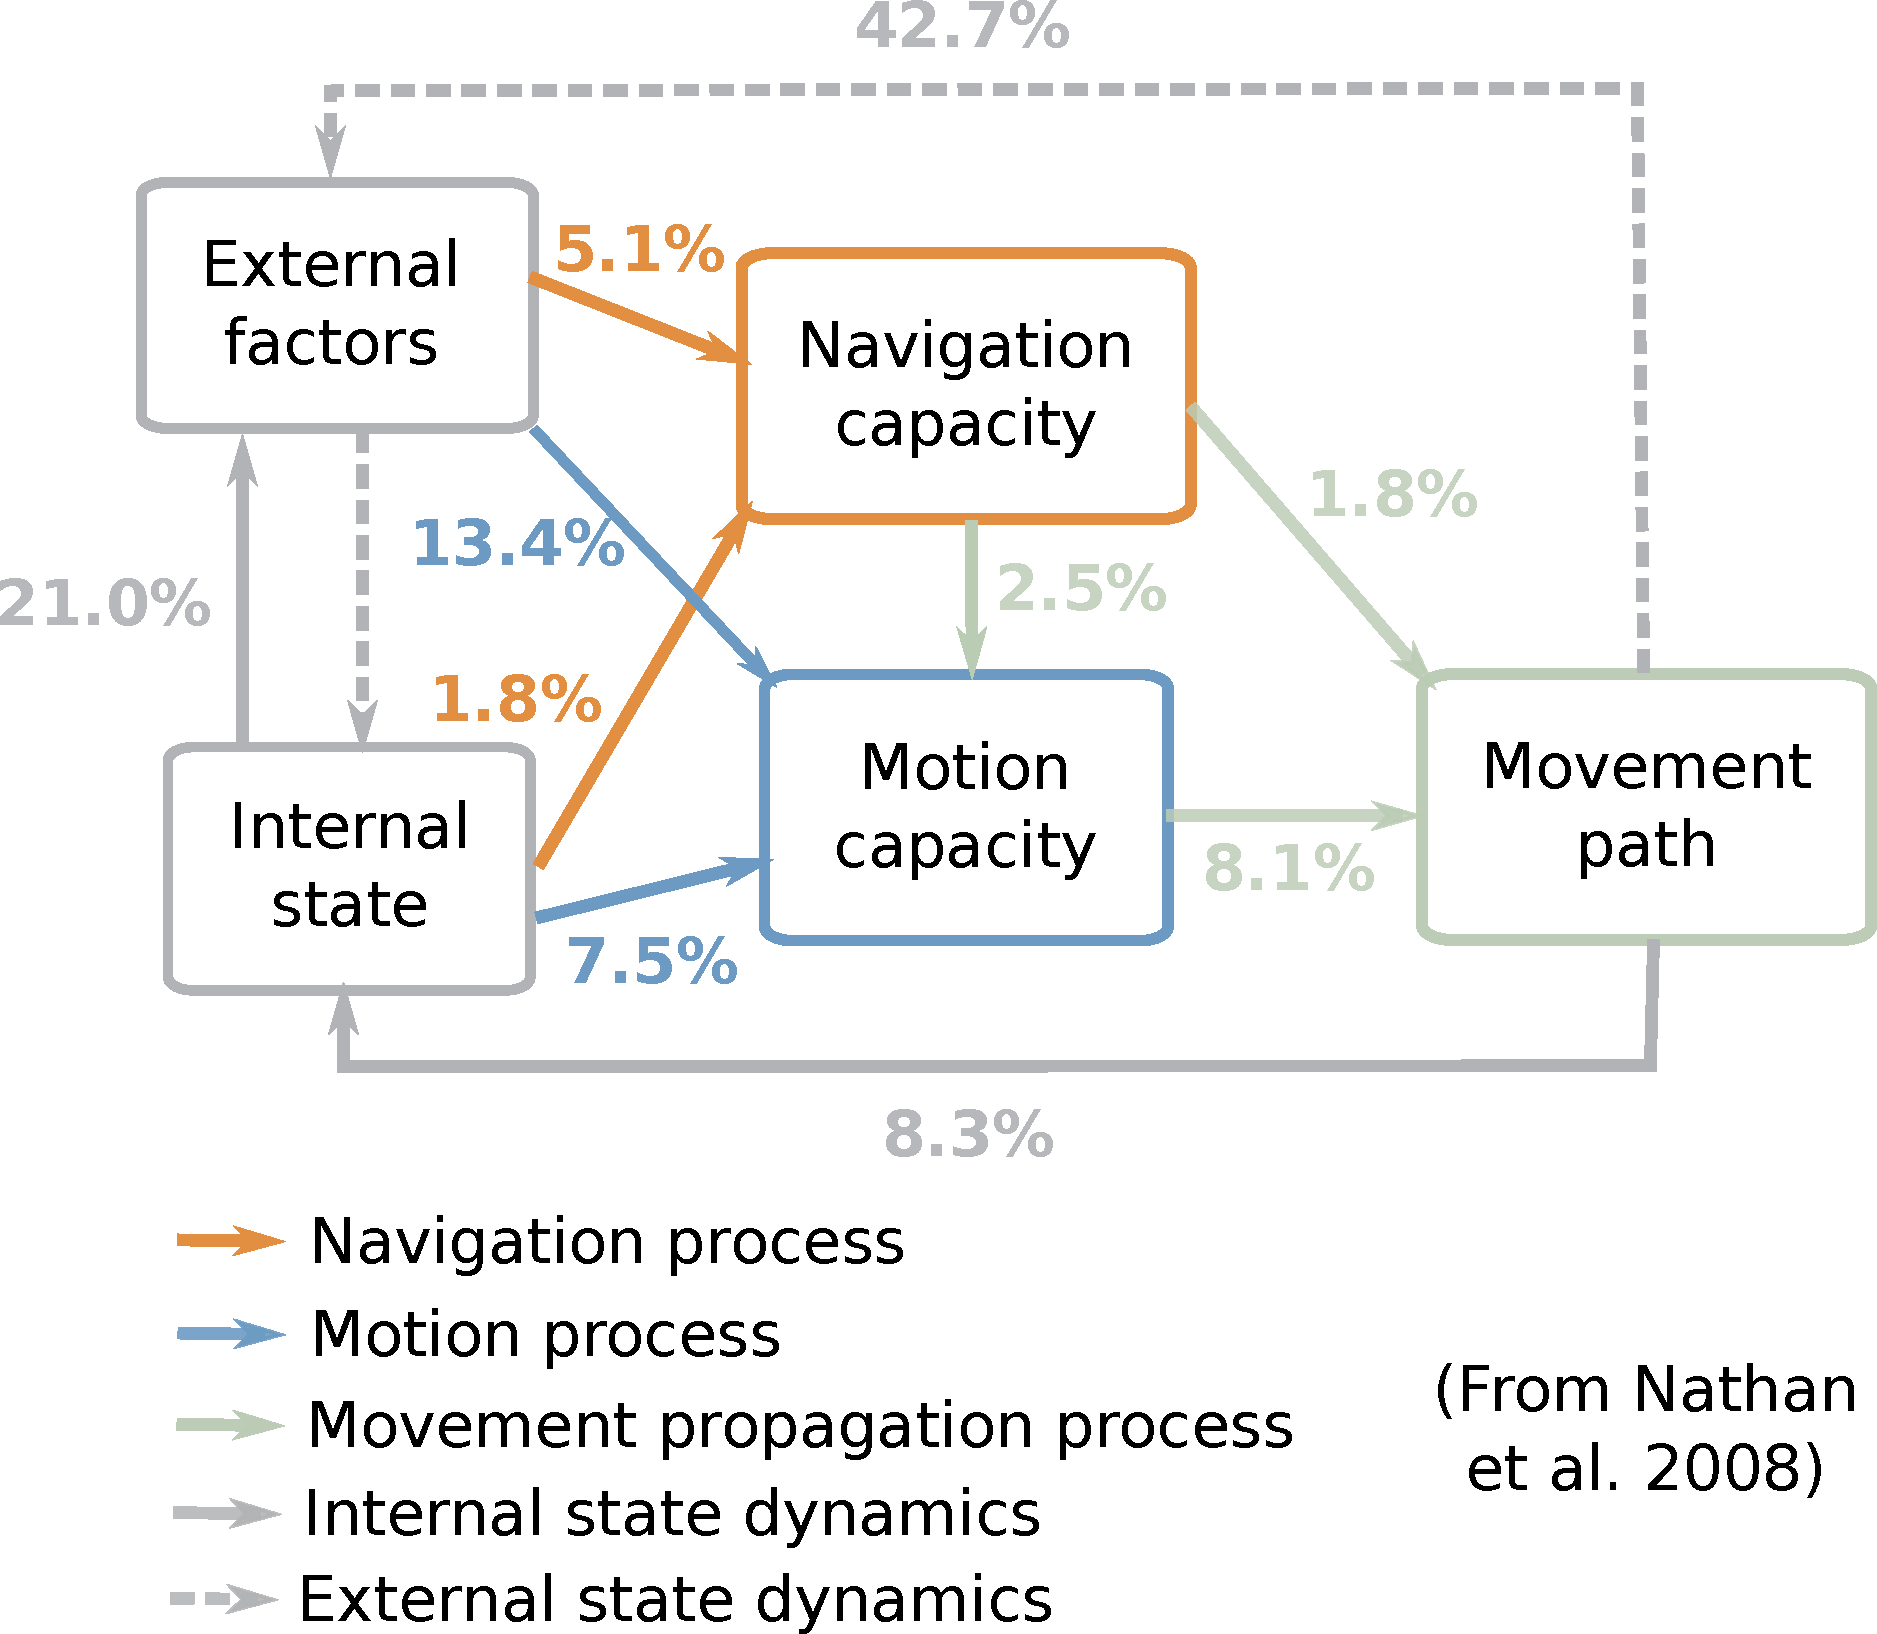
\includegraphics[width=.8\linewidth]{./img/MovEcoFrame.pdf}
\caption{Movement ecology paradigm (MPE) from Nathan et al. 2008. The values shown are the percentages of scientific papers (from which we extracted MPE information: 3750) that showed in the abstract that they were studying those components or links between components. Percentages in links with movement path correspond to papers only mentioning the components, which we infer is linked to movement (because those are movement papers). }
\label{fig:mpe}
\end{figure}

\subsection*{The species: are we focusing too much on some species?}

- One or two lines of introduction on species studies in movement ecology. Then explain that we studied taxas and orders.
- Fig. 3: Main figure: barplots of taxa. Smaller subfigures: barplots of orders (max 2 subfigures).
- Comment results on taxa. Mammals historically easier to tag. Development of tags (see next section) is enabling tagging other taxa. But not all mammals' movement are being studied. It's mostly carnivores and ungulates. Why? Easier to tag? Longer life? More money behind? Are they becoming target species to develop more knowledge on processes? That would mean checking the studies of the framework on those orders and compare with the global results. 
- Other orders worth mentioning? Are there more studies on navigation or motion for certain orders? Are the spatial distribution of authors different? Is there something we can say about fish?
- Studies on humans. [Ref1] mentions the study of humans should be included in movement ecology since they have effects in the dispersal of many organisms. Another paper (Thums et al 2018) discusses the potential of integrating human movement research in animal ecology (methods, software). Because of data availability, human research is developing platforms and methods to deal with big data, which is something that animal movement will need. Also, in the past, human movement studies have taken methods applied to animal movement first (e.g. random walk models). Here we included humans as the studied organisms; most of them analyzed as regular pedestrians or fishers \todo[color=blueish!20]{RJ: We don't have those results yet.} 
- So... why are we studying some organisms more than others? Does it make sense? Should we break the trend?
- Add stuff from the survey.

\begin{figure}%[tbhp]
\centering
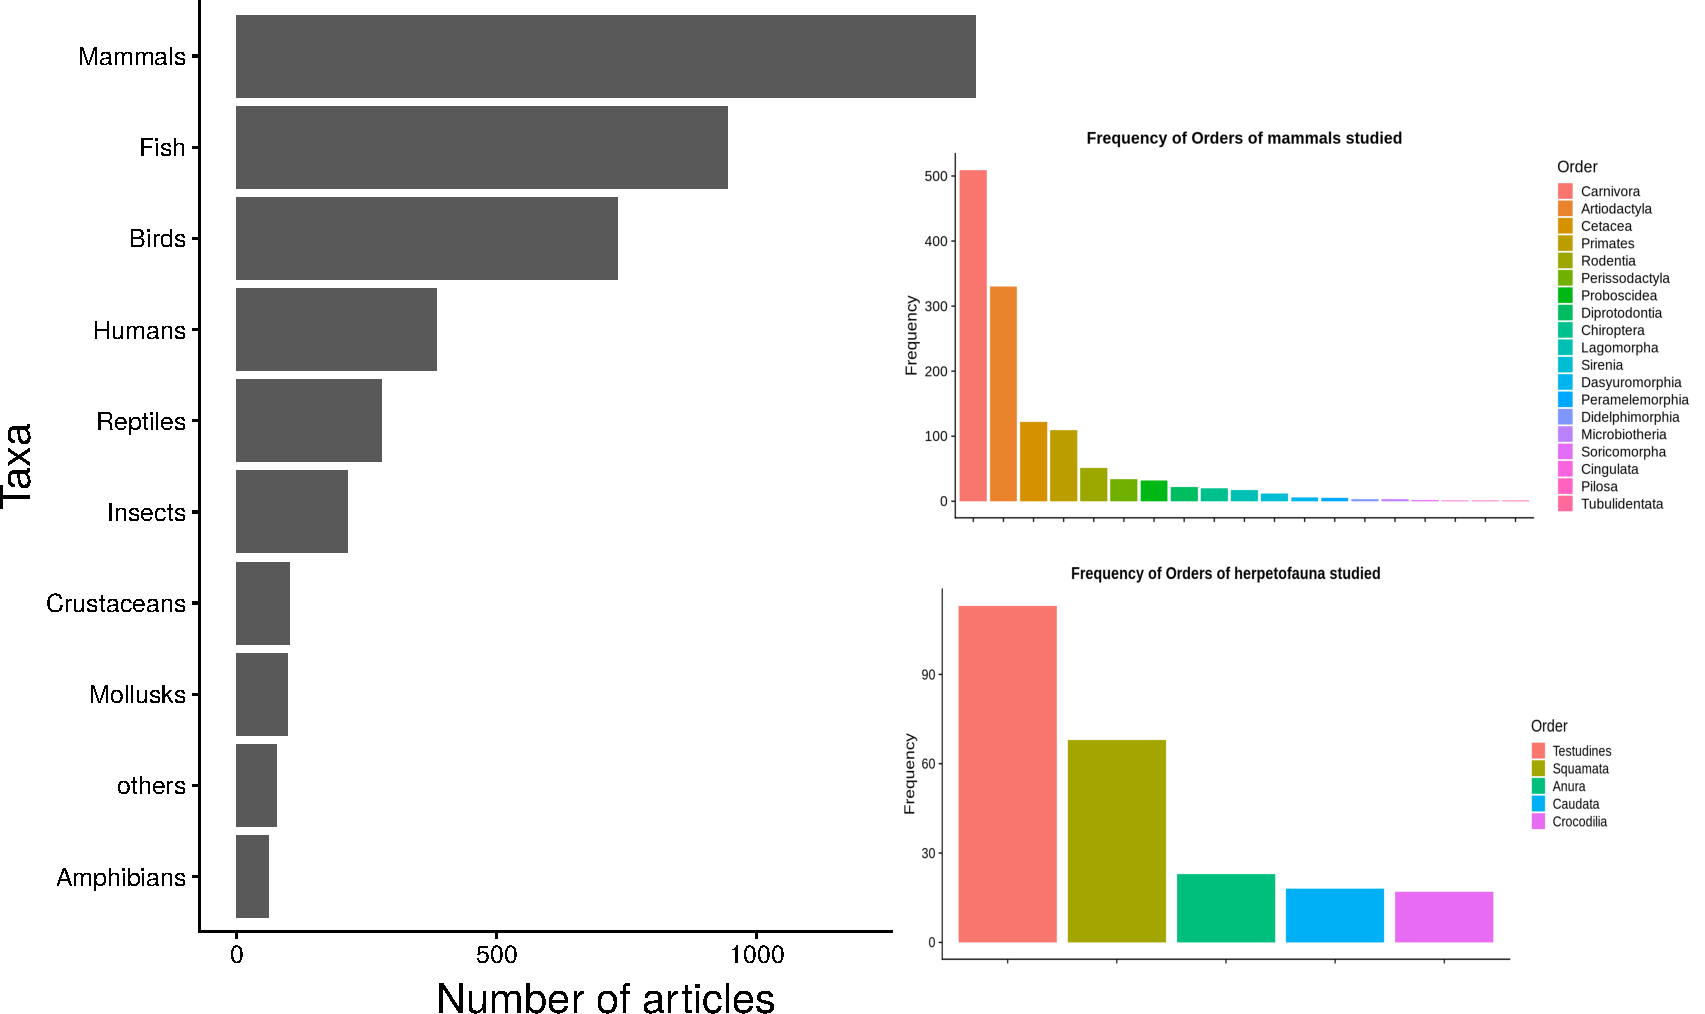
\includegraphics[width=.8\linewidth]{./img/Species.pdf}
\caption{Left: Barplots of frequency of taxa studies. Top right: Barplots of frequency of studies of mammal orders. Bottom right: Barplots of frequency of studies of reptile orders. Click on the file to see it better. }
\label{fig:species}
\end{figure}

\subsection*{Data collection: higher resolution to capture movement}

- One or two lines about tracking organisms and biologging. 
- Fig. 4: Ts of devices. 
- Check GPS and radio  \todo[color=blueish!20]{RJ: This reminds me that SP has to check weird results between orders and radio.} trade-off. Hebblewhite and Haydon (2010) offer a discussion on stuff we would be neglecting by choosing GPS instead of radar. 
- Talk about higher resolution for movement. Also shown by increasing use of accelerometer and video data. 
- What questions are these devices enabling to answer? What about the MEP? Or are we not collecting the right type of data yet? What do we want? Are the questions (i.e. MEP) playing a role in data collection planning? I think I read something about that in Hughey et al (2018) though not about MEP. 
- Also, by going for higher resolutions, are we neglecting larger scale movement?
- Remaining challenges in data collection. And even if we explore A LOT environmental factors role in movement, we still have the issue of having environmental data at different spatial and time scales than the movement data. How are we solving this?
- Data sharing and standardization. The repositories. Challenges for databases.
- What's next? (drones?) 
- Add stuff from the survey.

\begin{figure}%[tbhp]
\centering
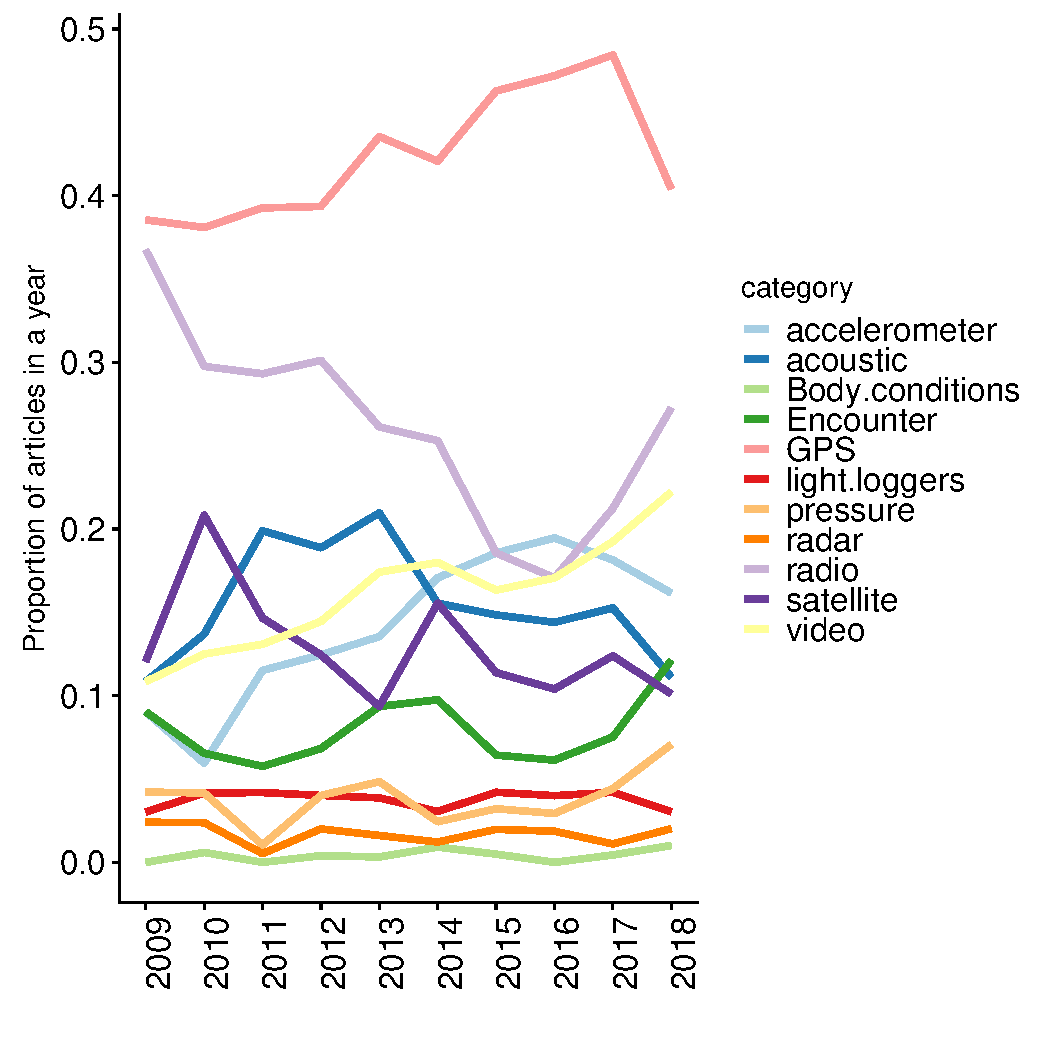
\includegraphics[width=.8\linewidth]{./img/devices_ts.pdf}
\caption{Proportion of articles (per year) mentioning each type of device.}
\label{fig:devices}
\end{figure}

\subsection*{Software: towards standardization and free access}

- One or two lines about software's importance for data processing and analysis, more now than before because of the volumes of data and the complexity of the methods. 
- Fig. 5: Ts of software. 
- Talk about software ts. Most software were never very much used (actually some French software are only used in French-speaking countries, see Supp. Mat. 3). The R trend which is a trend for standardization (everyone "speaking" the same language), not only in movement ecology but in science in general. Programming and also free access to codes will make science more reproducible. 
- Advantages and risks of everyone turning to R (talk about the packages and mention the R paper). 
- Emphasize need for integration and Ropensci as a peer-reviewed tool that forces packages to be developed for users. 
- Can other software appear in the near future? Python? I just read on the news that facebook and Google are trying to develop new software to satisfy big data needs.
- Add stuff from the survey.

\begin{figure}%[tbhp]
\centering
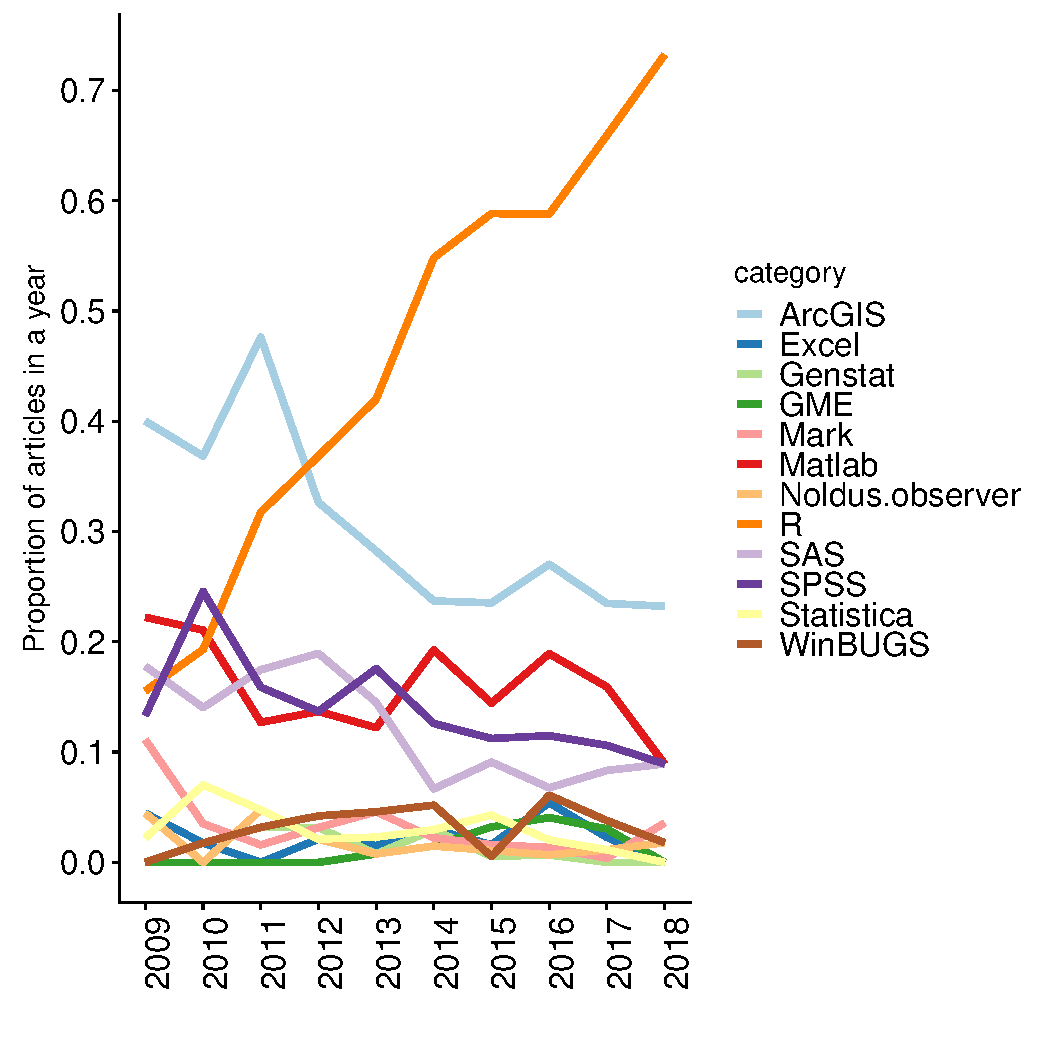
\includegraphics[width=.8\linewidth]{./img/software_ts.pdf}
\caption{Proportion of articles (per year) mentioning each software. Only the top 12 most used software are shown. For the complete frequency table go to Supp. Mat...4?}
\label{fig:software}
\end{figure}

\subsection*{Methods: from hypothesis testing to movement models}

- A phrase about methods being key to get from anecdotal observation to significant, representative scientific findings. Here we refer to statistical and mathematical methods; mostly statistical which are more common now (and the ones I know).
- Holyoak mentioned in his paper that most papers were about hypothesis testing. Here we should show our statistics confirming that for this decade as well. So this is still true. Are we p-value dependent? Short discussion about p-values; their usefulness and their danger (to find good p-values and feel happy and ready to publish). 
- There is not a unique way to classify methods, and many could fall into several categories at the same time. For instance, regression trees could be considered machine learning, a multivariate technique and a regression method (strictly speaking, any method with more than one variable would be multivariate). A random walk could be a time series method or a spatio-temporal method depending if it considers a 2 or 3D component or not. Moreover, it is difficult to directly and automatically link a method to the MEP. Several methods could be used for the same question, and the choice of method also depends on the available data (and the preference of the analyst). Here we propose a classification based on methodological questions for movement ecology analysis. 

Methodological questions would be: 1) Where, with a focus on spatial components; 2) why, focusing on identifying covariates that would explain the variable or process studied; 3) how, focused on the links between a variable and the others; 4) when, with a focus on the temporal dimension; 5) what, with the goal of identifying a latent variable (i.e. a behavioral pattern) that would be behind the observed movement patterns; and 6) with whom, focusing on the interspecific or conspecific interactions that would have an effect on movement. Table \ref{table:methods} summarizes these definitions with some mathematical notations and examples of methods that correspond to each question. A method could, however, be useful for several questions; for example, a hidden Markov model links a hidden variable (what) to observed variables (why) in time (when) via conditional probabilities (how). Here we identified $\sim 200$ statistical methods and identified the questions they can answer (Supp. Mat. 5?). 

\begin{table}%[tbhp]
\centering
\caption{Main methodological questions in movement ecology and variables involved}
\begin{tabular}{lcl}
Question   & Variables involved                  & Examples of methods                              \\
\midrule
Where?     & $X$; $f(X)$                         & Geostatistics, home range methods \\
Why?       & $Z \sim g(\mathbf{Z'})$             & Hypothesis tests                                 \\
How?       & $Z \sim \mathbf{g}(Z')$             & Mechanistic models                               \\
When?      & $t$; $f(t)$                         & Time series models                               \\
What?      & $Y \sim h(Z)$                       & Classification methods                           \\
With whom? & $g(z_{\mathbf{i}}, z_{\mathbf{j}})$ & Agent-based models       \\
 \bottomrule
\end{tabular}
\addtabletext{$t$ represents a time step and $X(t)$ a given location in time. A continuous georeferenced variable in time (e.g. turning angle) would be denoted by $Z_{x,t} := f(X_t)$. $Y$ is a latent variable that could be expressed as a function of $Z$. $g$ is a distance function between individuals $i$ and $j$.}
\label{table:methods}
\end{table}

Describe global results for the questions (Why: 1709, How: 	1515, When: 859, Where:	842, What: 363, With whom: 215). Show Table \ref{table:keywords-questions} with the main keywords for each question. Discuss that when and where methods are not much used. Instead, it's more about why and how, driven by mixed models. While there may be some versions of mixed models that properly consider spatial and temporal components, most of them don't or add them as simple covariates. \todo[color=blueish!20]{RJ: This is what I think but I may be completely wrong.} While it is good that researchers are using models (add here a statistic on how many abstracts use the word "model") not only to obtain a p-value (hopefully) but also to synthesize their knowledge of organisms' movement, since movement has a spatial and temporal component we should be movement towards more movement models. \todo[color=blueish!20]{RJ: Do you agree?} I need to quantify how many papers talk about movement models (so potentially spatiotemporal models like RWs, SSMs or HMMs). Also mention that there are several R packages for modeling movement. 
- Mention the reviews of methods for movement, mostly for movement models. Like Patterson et al. 2017.
- Some challenges? Continuous movement models are not quite there yet. Patterson's review and McClinctock et al. 2014. Do you see other challenges? 
- Add stuff from the survey.

\begin{table}%[tbhp]
\centering
\caption{Main methods for each question}
\begin{tabular}{llllllllllll}
Why & & How & & When & & What & & With whom & \\
\midrule
word                     & count & word                 & count & word                & count & word                   & count & word                                     & count & word                              & count \\
\midrule
random walk              & 282   & Akaike's information & 593   & mixed effects model & 483   & random walk            & 282   & \%SSM\%                                  & 168   & social network!sedentary          & 83    \\
density kernel           & 178   & \%ANOVA\%            & 511   & linear model        & 288   & movement model         & 172   & \%HMM\%                                  & 113   & individual-based model            & 82    \\
movement model           & 172   & mixed effects model  & 483   & random walk         & 282   & \%SSM\%                & 168   & Markov chain                             & 106   & agent-based model                 & 47    \\
minimum convex polygon   & 166   & t-test               & 311   & \%GLM\%             & 209   & \%HMM\%                & 113   & clustering analysis|clustering algorithm & 37    & \%SPP\%                           & 15    \\
utilization distribution & 141   & linear model         & 288   & regression model    & 202   & Markov chain           & 106   & K-means                                  & 33    & Individual-based simulation model & 14    \\
tortuosity               & 66    & \%GLM\%              & 209   & linear regression   & 192   & individual-based model & 82    & decision tree                            & 28    & relative phase                    & 14    \\
\%SSF\%                  & 63    & regression model     & 202   & logistic regression & 172   & Fourier                & 78    & random forest                            & 22    & network topology                  & 8     \\
Brownian motion          & 58    & linear regression    & 192   & movement model      & 172   & \%SSF\%                & 63    & classification tree                      & 15    & Pattern-oriented model            & 8     \\
\%BBMM\%                 & 52    & logistic regression  & 172   & \%SSM\%             & 168   & Brownian motion        & 58    & bcpa                                     & 14    & proximity index                   & 1     \\
sinuosity                & 37    & \%SSM\%              & 168   & \%RSF\%             & 140   & \%BBMM\%               & 52    & neural network                           & 13    & transfer entropy                  & 1    \\
\bottomrule
\end{tabular}
\addtabletext{I have to edit the calculations to pass from keywords to methods. Also, I have to filter model selection criteria. And... this doesn't fit. Ideas?}
\label{table:keywords-questions}
\end{table}

\subsection*{Interdisciplinarity for movement}

\todo[color=greenish!20,inline=TRUE]{RJ: I keep forgetting the differences between inter, multi and transdisciplinarity. Help?} 
- Movement ecology as a multidisciplinary field. If we want to understand movement processes better, we need ecologists, physiologists, statisticians, mathematicians, geophysicists, meteorologists, oceanographers, software engineers (am I forgetting some people?) to interact and push the field forward. 
- Here I should show results that I don't have yet on the diversity of journal with movement ecology papers, and on researchers' affiliations. 
- Imaginary table 3: it would show results on journals. I've got papers from 264 journals. We should come up with categories for classifications. How about ecology, biology, general, fisheries, methodological (mainly statistics, maths, data processing, GIS), physics (can oceanography be included here?), human (e.g. transportation, behavior research, human kinetics, sports). Does it make sense? Consider that this is to show if we are studying movement ecology from many disciplines. Also, I don't quite get the difference between ecology and biology so I need help with that (sorry). 

- Fig. \ref{fig:discip} would be composed of a map of affiliations and blocks of 'professions' (ecologist, biologist, physicist, stat/mathematician) and a quantification of their interactions. Like in the example.
\begin{figure}%[tbhp]
\centering
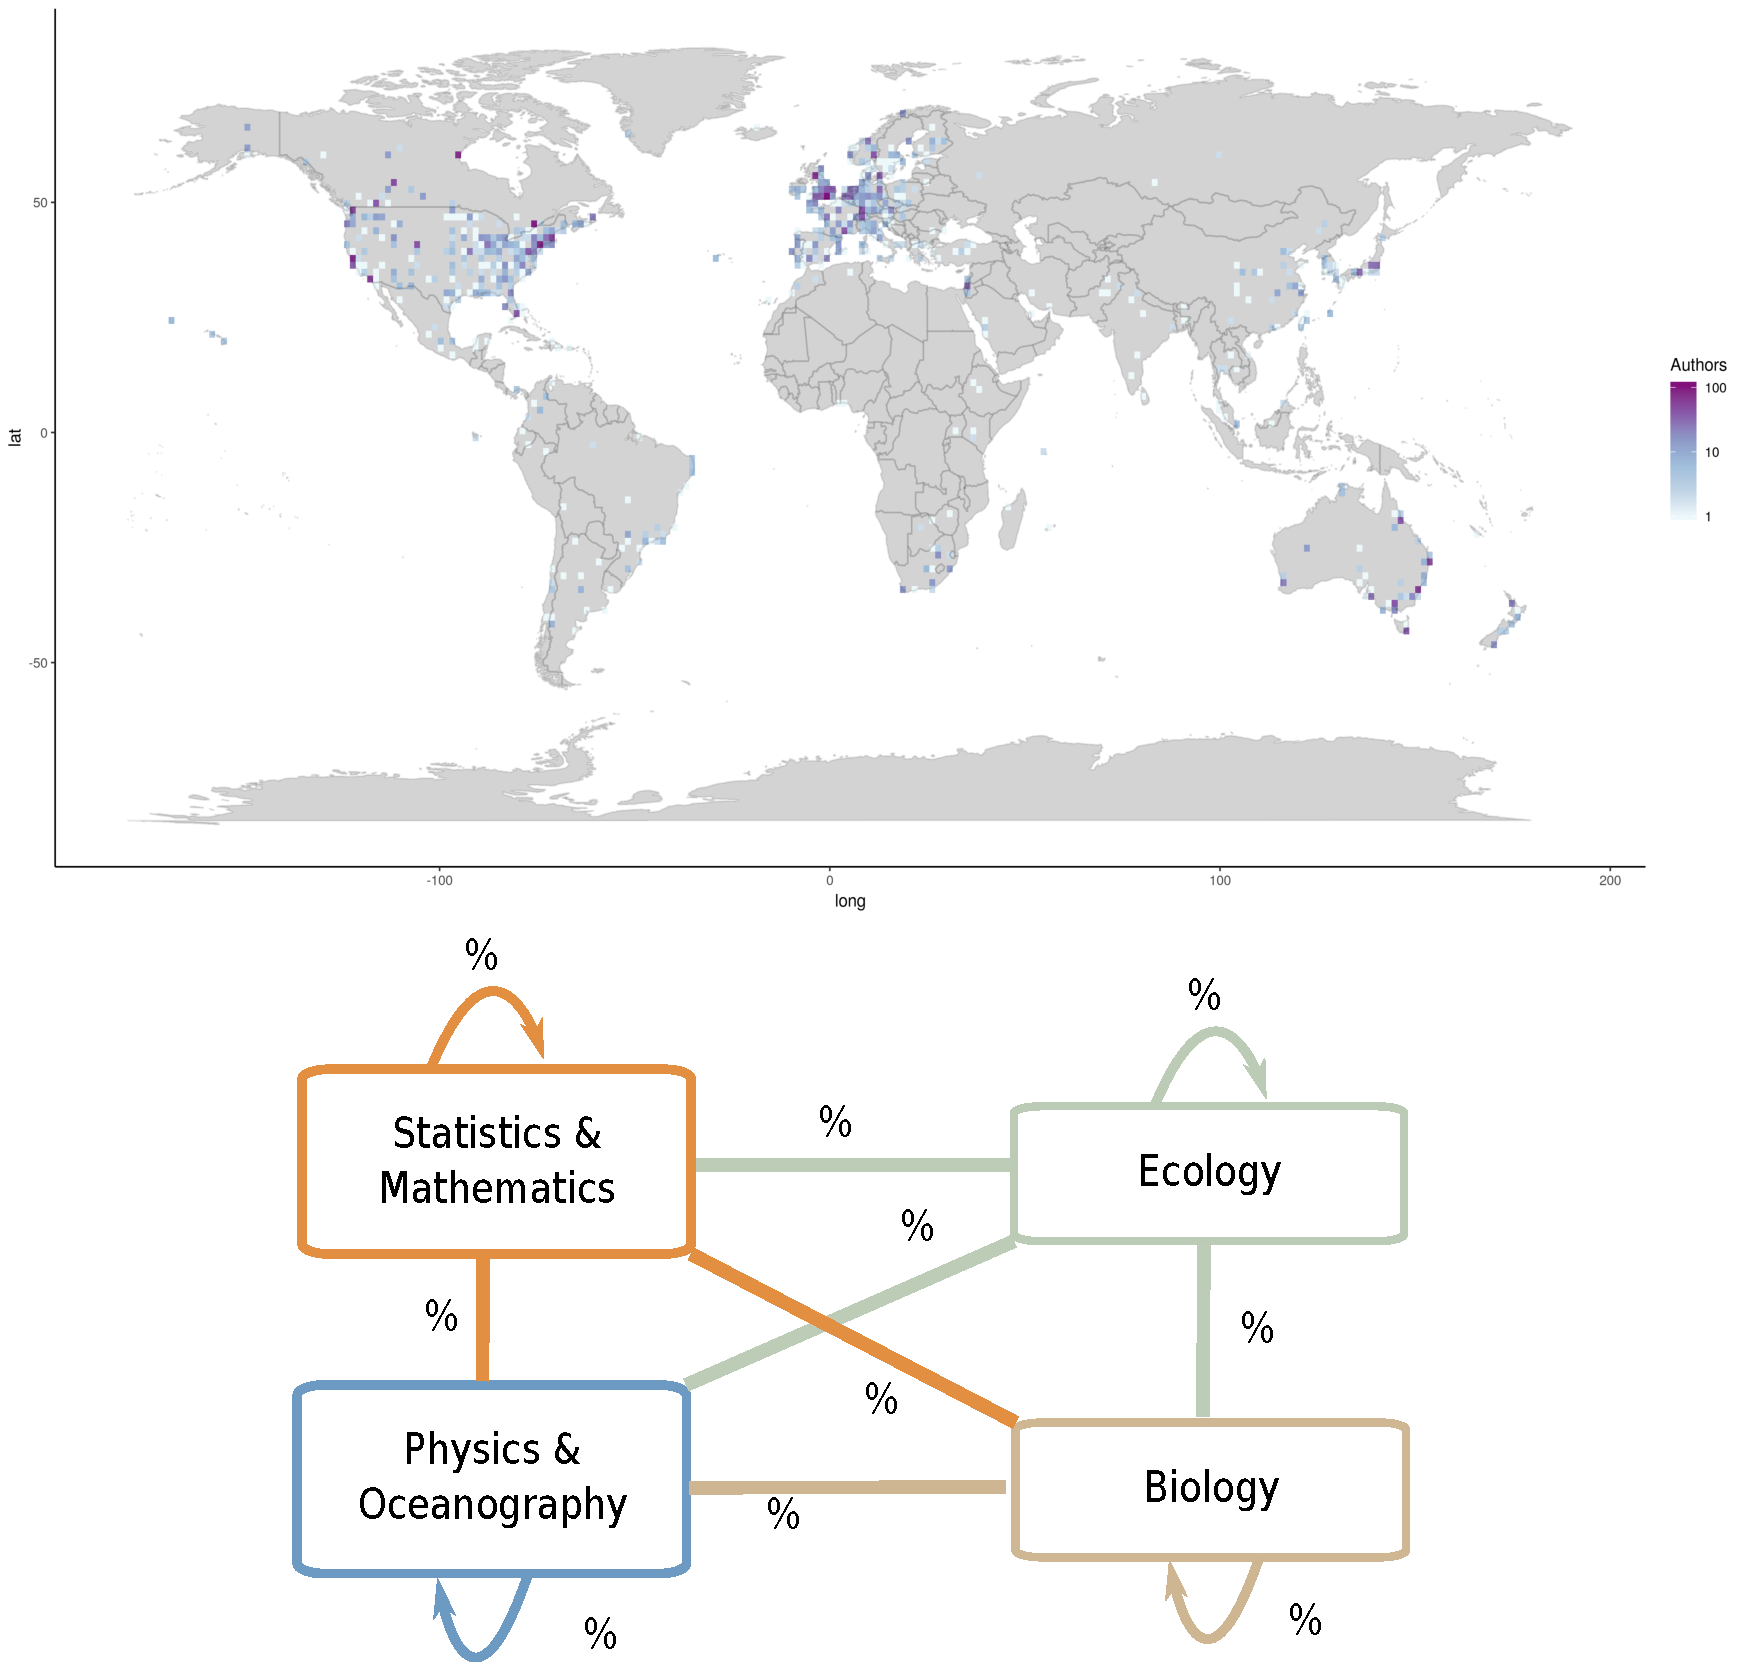
\includegraphics[width=.9\linewidth]{./img/interdiscip.pdf}
\caption{Movement ecologists. Top: spatial distribution of authors of movement ecology papers. Bottom: interactions between researchers from different fields based on coauthorship.}
\label{fig:discip}
\end{figure}

- Discuss results. Are we interacting more than before? Is it still an issue? What's missing? Talk about conferences of biologging or movement ecology. Also ISEC and... biometrics? Ecological conferences (are the other people going?). 

\subsection*{Movement ecology for management and conservation}

This is the only application I found from the topics results (and the only way I found to add some of the topics results). We would show that among topics, this is the most popular one (Table in Supp. Mat), so there are efforts to respond to management and conservation needs with movement analysis. There is actually framework proposed by Allen and Singh (2016) to link movement ecology and wildlife management and conservation. Studies mention some challenges to actually go to manag. and conserv. such as team work with stakeholders, accesss to data of several species since management has to consider interactions in the ecosystem... so actually improving every single aspect of movement ecology that we've mentioned here could help for management and conservation. I should also mention somewhere the paper of Fraser et al (2018) comparing overall studies of movement ecology with actual use of them for conservation (but their study makes no sense by searching for "movement ecology" in any part of the text of a paper).

\subsection*{Summary: future directions}

Wrapping up. No idea of what to put here. Oh, yeah: add stuff from the survey.


% FYI:

% [1]A. M. Allen and N. J. Singh, “Linking Movement Ecology with Wildlife Management and Conservation,” Front. Ecol. Evol., vol. 3, 2016.
% [2]M. Baguette, V. M. Stevens, and J. Clobert, “The pros and cons of applying the movement ecology paradigm for studying animal dispersal,” Movement Ecology, vol. 2, no. 1, p. 13, Jul. 2014.
% [3]L. Börger, “EDITORIAL: Stuck in motion? Reconnecting questions and tools in movement ecology,” Journal of Animal Ecology, vol. 85, no. 1, pp. 5–10, 2016.
% [4]H. A. Campbell, F. Urbano, S. Davidson, H. Dettki, and F. Cagnacci, “A plea for standards in reporting data collected by animal-borne electronic devices,” Animal Biotelemetry, vol. 4, no. 1, p. 1, Jan. 2016.
% [5]S. J. Cooke et al., “Biotelemetry: a mechanistic approach to ecology,” Trends in Ecology & Evolution, vol. 19, no. 6, pp. 334–343, Jun. 2004.
% [6]G. S. Cumming, N. Gaidet, and M. Ndlovu, “Towards a unification of movement ecology and biogeography: conceptual framework and a case study on Afrotropical ducks,” Journal of Biogeography, vol. 39, no. 8, pp. 1401–1411, 2012.
% [7]F. J. Dyson, “Is Science Mostly Driven by Ideas or by Tools?,” Science, vol. 338, no. 6113, pp. 1426–1427, Dec. 2012.
% [8]K. C. Fraser, K. T. A. Davies, C. M. Davy, A. T. Ford, D. T. T. Flockhart, and E. G. Martins, “Tracking the Conservation Promise of Movement Ecology,” Front. Ecol. Evol., vol. 6, 2018.
% [9]M. Hebblewhite and D. T. Haydon, “Distinguishing technology from biology: a critical review of the use of GPS telemetry data in ecology,” Philos Trans R Soc Lond B Biol Sci, vol. 365, no. 1550, pp. 2303–2312, Jul. 2010.
% [10]M. Holyoak, R. Casagrandi, R. Nathan, E. Revilla, and O. Spiegel, “Trends and missing parts in the study of movement ecology,” PNAS, vol. 105, no. 49, pp. 19060–19065, Dec. 2008.
% [11]T.-Y. Huang, B. Zhao, S.-Q. Dai, H. Li, J. Ma, and X.-M. Xiao, “Different nation, different ecology: Comparison of ecological research features in China and the US during the recent three decades,” Global Ecology and Conservation, vol. 16, p. e00509, Oct. 2018.
% [12]Hughey Lacey F., Hein Andrew M., Strandburg-Peshkin Ariana, and Jensen Frants H., “Challenges and solutions for studying collective animal behaviour in the wild,” Philosophical Transactions of the Royal Society B: Biological Sciences, vol. 373, no. 1746, p. 20170005, May 2018.
% [13]F. Jeltsch et al., “Integrating movement ecology with biodiversity research - exploring new avenues to address spatiotemporal biodiversity dynamics,” Movement Ecology, vol. 1, no. 1, p. 6, Aug. 2013.
% [14]S. K. Lowerre-Barbieri, R. Kays, J. T. Thorson, and M. Wikelski, “The ocean’s movescape: fisheries management in the bio-logging decade (2018–2028),” ICES J Mar Sci.
% [15]E. McCallen, J. Knott, G. Nunez‐Mir, B. Taylor, I. Jo, and S. Fei, “Trends in ecology: shifts in ecological research themes over the past four decades,” Frontiers in Ecology and the Environment, vol. 0, no. 0.
% [16]K. Morelle, F. Lehaire, and P. Lejeune, “Is wild boar heading towards movement ecology? A review of trends and gaps,” Wildlife Biology, vol. 20, no. 4, pp. 196–205, Aug. 2014.
% [17]K. Morelle, T. Podgórski, C. Prévot, O. Keuling, F. Lehaire, and P. Lejeune, “Towards understanding wild boar Sus scrofa movement: a synthetic movement ecology approach,” Mammal Review, vol. 45, no. 1, pp. 15–29, Jan. 2015.
% [18]R. Nathan, “An emerging movement ecology paradigm,” PNAS, vol. 105, no. 49, pp. 19050–19051, Dec. 2008.
% [19]R. Nathan et al., “A movement ecology paradigm for unifying organismal movement research,” PNAS, vol. 105, no. 49, pp. 19052–19059, Dec. 2008.
% [20]M. B. Ogburn, A.-L. Harrison, F. G. Whoriskey, S. J. Cooke, J. E. Mills Flemming, and L. G. Torres, “Addressing Challenges in the Application of Animal Movement Ecology to Aquatic Conservation and Management,” Front. Mar. Sci., vol. 4, 2017.
% [21]W. A. Reiners, J. A. Lockwood, D. S. Reiners, and S. D. Prager, “100 years of ecology: what are our concepts and are they useful?,” Ecological Monographs, vol. 87, no. 2, pp. 260–277, 2017.
% [22]E. J. Sayer, “The anatomy of an excellent review paper,” Functional Ecology, vol. 32, no. 10, pp. 2278–2281, Oct. 2018.
% [23]I. K. Shimatani, K. Yoda, N. Katsumata, and K. Sato, “Toward the Quantification of a Conceptual Framework for Movement Ecology Using Circular Statistical Modeling,” PLoS ONE, vol. 7, no. 11, 2012.
% [24]W. J. Sutherland et al., “Identification of 100 fundamental ecological questions,” Journal of Ecology, vol. 101, no. 1, pp. 58–67, 2013.
% [25]Tomkiewicz Stanley M., Fuller Mark R., Kie John G., and Bates Kirk K., “Global positioning system and associated technologies in animal behaviour and ecological research,” Philosophical Transactions of the Royal Society B: Biological Sciences, vol. 365, no. 1550, pp. 2163–2176, Jul. 2010.
% Thums, M., Fernández-Gracia, J., Sequeira, A. M. M., Eguíluz, V. M., Duarte, C. M., & Meekan, M. G. (2018). How Big Data Fast Tracked Human Mobility Research and the Lessons for Animal Movement Ecology. Frontiers in Marine Science, 5. https://doi.org/10.3389/fmars.2018.00021


% \subsection*{List of figures and tables}
% Fig.1: double time series of papers (in movement ecology and in science)
% Fig.2: schematic representation of the aspects of movement ecology reviewed here
% Fig.3: MPE links
% Fig.4: Barplots of taxa and orders
% Fig.5: ts of devices
% Fig.6: ts of software
% Fig.7: map and discipline interaction boxes
% Table 1: most common keywords in each MPE component
% Table 2: most common keywords in each methodological questions
% Table 3: frequency of types of journals (by discipline)

% % \subsection*{Manuscript Length}

% % PNAS generally uses a two-column format averaging 67 characters, including spaces, per line. The maximum length of a Direct Submission research article is six pages and a Direct Submission Plus research article is ten pages including all text, spaces, and the number of characters displaced by figures, tables, and equations.  When submitting tables, figures, and/or equations in addition to text, keep the text for your manuscript under 39,000 characters (including spaces) for Direct Submissions and 72,000 characters (including spaces) for Direct Submission Plus.

% % \subsection*{References}

% % References should be cited in numerical order as they appear in text; this will be done automatically via bibtex, e.g. \cite{belkin2002using} and \cite{berard1994embedding,coifman2005geometric}. All references should be included in the main manuscript file.  

% % \subsection*{Data Archival}

% % PNAS must be able to archive the data essential to a published article. Where such archiving is not possible, deposition of data in public databases, such as GenBank, ArrayExpress, Protein Data Bank, Unidata, and others outlined in the Information for Authors, is acceptable.

% % \subsection*{Language-Editing Services}
% % Prior to submission, authors who believe their manuscripts would benefit from professional editing are encouraged to use a language-editing service (see list at www.pnas.org/site/authors/language-editing.xhtml). PNAS does not take responsibility for or endorse these services, and their use has no bearing on acceptance of a manuscript for publication. 




% % \begin{SCfigure*}[\sidecaptionrelwidth][t]
% % \centering
% % 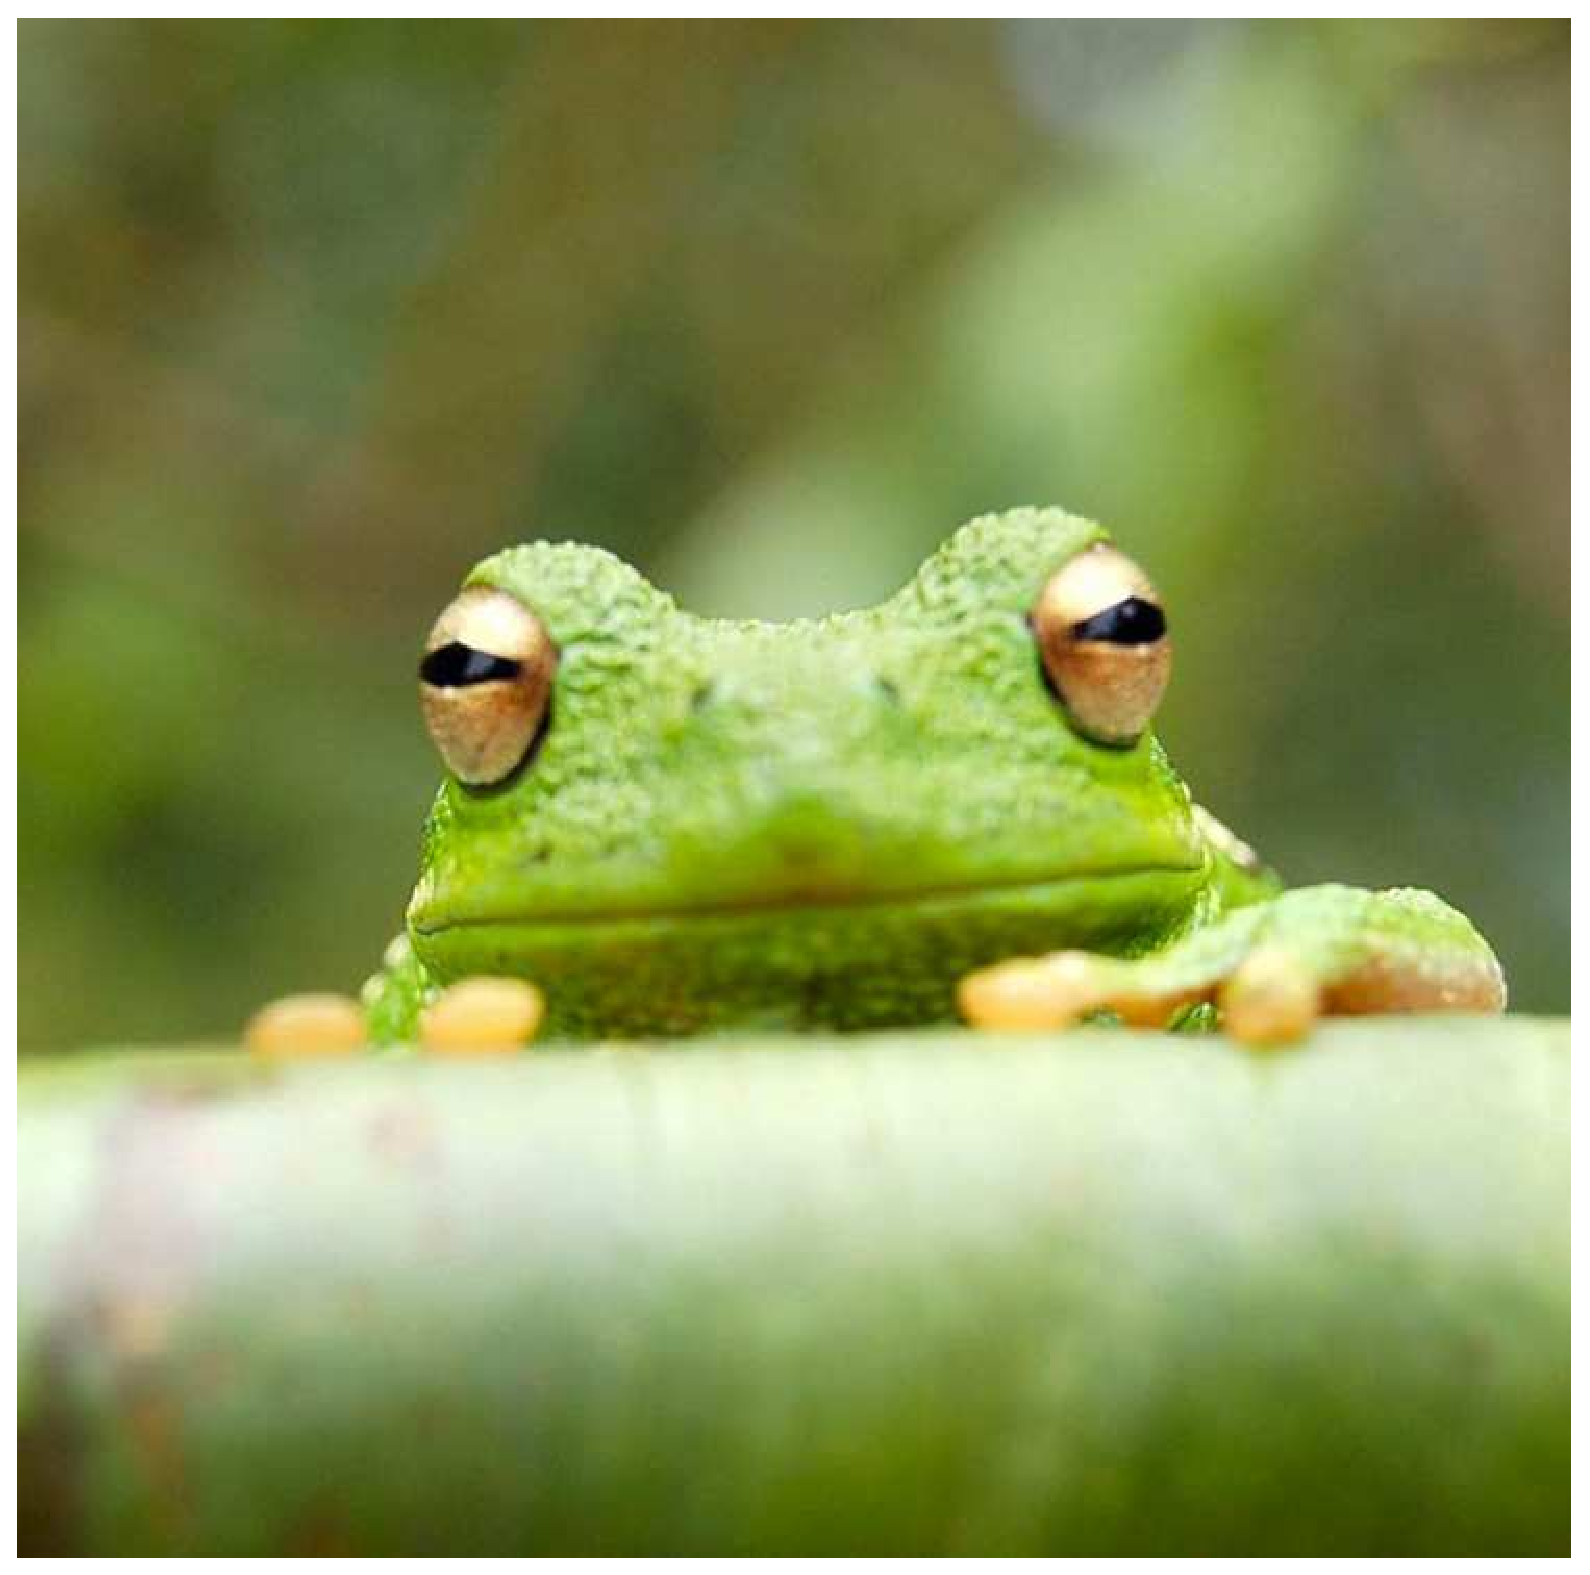
\includegraphics[width=11.4cm,height=11.4cm]{frog}
% % \caption{This caption would be placed at the side of the figure, rather than below it.}\label{fig:side}
% % \end{SCfigure*}

% % \subsection*{Digital Figures}

% % Only TIFF, EPS, and high-resolution PDF for Mac or PC are allowed for figures that will appear in the main text, and images must be final size. Authors may submit U3D or PRC files for 3D images; these must be accompanied by 2D representations in TIFF, EPS, or high-resolution PDF format.  Color images must be in RGB (red, green, blue) mode. Include the font files for any text. 

% % Figures and Tables should be labelled and referenced in the standard way using the \verb|\label{}| and \verb|\ref{}| commands.

% % Figure \ref{fig:frog} shows an example of how to insert a column-wide figure. To insert a figure wider than one column, please use the \verb|\begin{figure*}...\end{figure*}| environment. Figures wider than one column should be sized to 11.4 cm or 17.8 cm wide. Use \verb|\begin{SCfigure*}...\end{SCfigure*}| for a wide figure with side captions.

% % \subsection*{Tables}
% % In addition to including your tables within this manuscript file, PNAS requires that each table be uploaded to the submission separately as a “Table” file.  Please ensure that each table .tex file contains a preamble, the \verb|\begin{document}| command, and the \verb|\end{document}| command. This is necessary so that the submission system can convert each file to PDF.

% % \subsection*{Single column equations}

% % Authors may use 1- or 2-column equations in their article, according to their preference.

% % To allow an equation to span both columns, use the \verb|\begin{figure*}...\end{figure*}| environment mentioned above for figures.

% % Note that the use of the \verb|widetext| environment for equations is not recommended, and should not be used. 

% % \begin{figure*}[bt!]
% % \begin{align*}
% % (x+y)^3&=(x+y)(x+y)^2\\
% %       &=(x+y)(x^2+2xy+y^2) \numberthis \label{eqn:example} \\
% %       &=x^3+3x^2y+3xy^3+x^3. 
% % \end{align*}
% % \end{figure*}


% % \begin{table}%[tbhp]
% % \centering
% % \caption{Comparison of the fitted potential energy surfaces and ab initio benchmark electronic energy calculations}
% % \begin{tabular}{lrrr}
% % Species & CBS & CV & G3 \\
% % \midrule
% % 1. Acetaldehyde & 0.0 & 0.0 & 0.0 \\
% % 2. Vinyl alcohol & 9.1 & 9.6 & 13.5 \\
% % 3. Hydroxyethylidene & 50.8 & 51.2 & 54.0\\
% % \bottomrule
% % \end{tabular}

% % \addtabletext{nomenclature for the TSs refers to the numbered species in the table.}
% % \end{table}

% % \subsection*{Supporting Information (SI)}

% % Authors should submit SI as a single separate PDF file, combining all text, figures, tables, movie legends, and SI references.  PNAS will publish SI uncomposed, as the authors have provided it.  Additional details can be found here: \href{http://www.pnas.org/page/authors/journal-policies}{policy on SI}.  For SI formatting instructions click \href{https://www.pnascentral.org/cgi-bin/main.plex?form_type=display_auth_si_instructions}{here}.  The PNAS Overleaf SI template can be found \href{https://www.overleaf.com/latex/templates/pnas-template-for-supplementary-information/wqfsfqwyjtsd}{here}.  Refer to the SI Appendix in the manuscript at an appropriate point in the text. Number supporting figures and tables starting with S1, S2, etc.

% % Authors who place detailed materials and methods in an SI Appendix must provide sufficient detail in the main text methods to enable a reader to follow the logic of the procedures and results and also must reference the SI methods. If a paper is fundamentally a study of a new method or technique, then the methods must be described completely in the main text.

% % \subsubsection*{SI Datasets} 

% % Supply Excel (.xls), RTF, or PDF files. This file type will be published in raw format and will not be edited or composed.


% % \subsubsection*{SI Movies}

% % Supply Audio Video Interleave (avi), Quicktime (mov), Windows Media (wmv), animated GIF (gif), or MPEG files and submit a brief legend for each movie in a Word or RTF file. All movies should be submitted at the desired reproduction size and length. Movies should be no more than 10 MB in size.


% % \subsubsection*{3D Figures}

% % Supply a composable U3D or PRC file so that it may be edited and composed. Authors may submit a PDF file but please note it will be published in raw format and will not be edited or composed.


\matmethods{Please describe your materials and methods here. This can be more than one paragraph, and may contain subsections and equations as required. Authors should include a statement in the methods section describing how readers will be able to access the data in the paper. 

\subsection*{Subsection for Method}
Example text for subsection.
% \todo[color=greenish!20,inline=TRUE]{RJ: The structure for this section was in my notebook... I'll add it later.} 
}

\showmatmethods{} % Display the Materials and Methods section

\acknow{Please include your acknowledgments here, set in a single paragraph. Please do not include any acknowledgments in the Supporting Information, or anywhere else in the manuscript.}

\showacknow{} % Display the acknowledgments section

% Bibliography
\bibliography{pnas-sample}


\end{document}